\documentclass[border=10pt]{standalone}
\usepackage{tikz}

\def\D{\mathcal{D}} 
\def\C{\mathcal{C}} 
\def\X{\mathcal{X}}  
\def\O{\mathcal{O}}
\def\B{\mathcal{B}}
\def\J{\mathcal{J}}
\def\V{\mathcal{V}}
\def\S{\mathcal{S}}
\def\I{\mathcal{I}}
\def\L{\mathcal{L}}
\def\K{\mathcal{K}}
\def\Z{\mathcal{Z}}
\def\T{\mathcal{T}}
\def\F{\mathcal{F}}
\def\U{\mathcal{U}}

\begin{document}
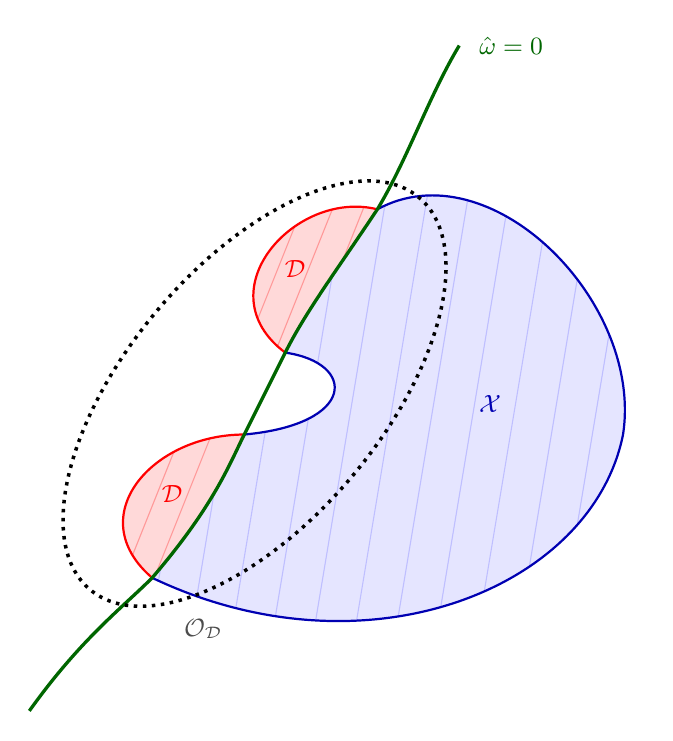
\begin{tikzpicture}[scale=1.3]

  % === TOPOLOGY ===
  % Green curve crosses outer boundary at 4 points:
  %   A  = (-1.8, -1.2)  bottom entry
  %   P2 = (-0.9,  0.2)  boundary crosses from left to right
  %   P3 = (-0.5,  1.0)  boundary crosses from right to left
  %   B  = ( 0.4,  2.4)  top exit
  %
  % Outer boundary segments:
  %   A→P2  : left arc  (red, lower D boundary)
  %   P2→P3 : crossing arc going RIGHT of green (blue, z boundary)
  %   P3→B  : left arc  (red, upper D boundary)
  %   B→A   : right arc (blue, z boundary)

  % =============================================
  % STEP 1: Fill z region
  %   green(A→P2) + crossing-arc(P2→P3) + green(P3→B) + right-arc(B→A)
  % =============================================
  \fill[blue!10]
    (-1.8,-1.2) .. controls (-1.2,-0.5) and (-1.05,-0.1) .. (-0.9,0.2)
    .. controls (0.2,0.3) and (0.2,0.9) .. (-0.5,1.0)
    .. controls (-0.3,1.4) and (0.0,1.8) .. (0.4,2.4)
    .. controls (1.5,3.0) and (3.0,1.5) .. (2.8,0.2)
    .. controls (2.5,-1.3) and (0.3,-2.2) .. (-1.8,-1.2)
    -- cycle;
  % z hatching
  \begin{scope}
    \clip
      (-1.8,-1.2) .. controls (-1.2,-0.5) and (-1.05,-0.1) .. (-0.9,0.2)
      .. controls (0.2,0.3) and (0.2,0.9) .. (-0.5,1.0)
      .. controls (-0.3,1.4) and (0.0,1.8) .. (0.4,2.4)
      .. controls (1.5,3.0) and (3.0,1.5) .. (2.8,0.2)
      .. controls (2.5,-1.3) and (0.3,-2.2) .. (-1.8,-1.2) -- cycle;
    \foreach \i in {-3,-2.6,...,4} {
      \draw[blue!25, thin] (\i,-4) -- (\i+1.5,5);
    }
  \end{scope}

  % =============================================
  % STEP 2: Fill lower D
  %   left-arc(A→P2) + green-reversed(P2→A)
  % =============================================
  \fill[red!15]
    (-1.8,-1.2) .. controls (-2.5,-0.6) and (-1.8,0.2) .. (-0.9,0.2)
    .. controls (-1.05,-0.1) and (-1.2,-0.5) .. (-1.8,-1.2)
    -- cycle;
  % lower D hatching
  \begin{scope}
    \clip
      (-1.8,-1.2) .. controls (-2.5,-0.6) and (-1.8,0.2) .. (-0.9,0.2)
      .. controls (-1.05,-0.1) and (-1.2,-0.5) .. (-1.8,-1.2) -- cycle;
    \foreach \i in {-4,-3.7,...,0} {
      \draw[red!40, thin] (\i,-3) -- (\i+2,2);
    }
  \end{scope}

  % =============================================
  % STEP 3: Fill upper D
  %   green(P3→B) + left-arc-reversed(B→P3)
  % =============================================
  \fill[red!15]
    (-0.5,1.0) .. controls (-0.3,1.4) and (0.0,1.8) .. (0.4,2.4)
    .. controls (-0.4,2.6) and (-1.3,1.6) .. (-0.5,1.0)
    -- cycle;
  % upper D hatching
  \begin{scope}
    \clip
      (-0.5,1.0) .. controls (-0.3,1.4) and (0.0,1.8) .. (0.4,2.4)
      .. controls (-0.4,2.6) and (-1.3,1.6) .. (-0.5,1.0) -- cycle;
    \foreach \i in {-2,-1.7,...,1} {
      \draw[red!40, thin] (\i,-1) -- (\i+2,4);
    }
  \end{scope}

  % =============================================
  % STEP 4: Draw outer boundary
  % =============================================
  % Red: lower left arc A → P2
  \draw[red, thick]
    (-1.8,-1.2) .. controls (-2.5,-0.6) and (-1.8,0.2) .. (-0.9,0.2);
  % Blue: crossing arc P2 → P3 (goes right of green)
  \draw[blue!70!black, thick]
    (-0.9,0.2) .. controls (0.2,0.3) and (0.2,0.9) .. (-0.5,1.0);
  % Red: upper left arc P3 → B
  \draw[red, thick]
    (-0.5,1.0) .. controls (-1.3,1.6) and (-0.4,2.6) .. (0.4,2.4);
  % Blue: right arc B → A
  \draw[blue!70!black, thick]
    (0.4,2.4) .. controls (1.5,3.0) and (3.0,1.5) .. (2.8,0.2)
              .. controls (2.5,-1.3) and (0.3,-2.2) .. (-1.8,-1.2);

  % =============================================
  % STEP 5: Green curve (on top of everything)
  % =============================================
  \draw[green!40!black, very thick]
    (-3.0,-2.5) .. controls (-2.5,-1.8) and (-2.1,-1.5) .. (-1.8,-1.2)
                .. controls (-1.2,-0.5) and (-1.05,-0.1) .. (-0.9,0.2)
                .. controls (-0.8,0.4) and (-0.6,0.8) .. (-0.5,1.0)
                .. controls (-0.3,1.4) and (0.0,1.8) .. (0.4,2.4)
                .. controls (0.7,2.9) and (0.9,3.5) .. (1.2,4.0);

  % =============================================
  % STEP 5.5: Dotted ellipse circling both D regions
  % =============================================
  \begin{scope}[rotate around={-40:(-0.80, 0.6)}]
    \draw[dotted, thick, line width=1.27pt] (-0.80, 0.6) ellipse (1.25 and 2.5);
  \end{scope}

  % =============================================
  % STEP 6: Labels
  % =============================================
  \node[green!40!black, right, font=\small] at (1.3, 4.0) {$\hat{\omega}=0$};
  \node[blue!70!black, font=\small] at (1.5, 0.5) {$\X$};
  \node[white!30!black, font=\small] at (-1.3, -1.7) {$\O_\D$};
  \node[red, font=\small, anchor=north west] at (-1.8, -0.2) {$\D$};
  \node[red, font=\small, anchor=north west] at (-0.6, 2.0) {$\D$};

\end{tikzpicture}
\end{document}
